\documentclass{article}
\usepackage{graphicx}
\usepackage{amsmath}
\usepackage{caption}
\usepackage{subcaption}
\usepackage{float}
\usepackage{biblatex}
\usepackage{booktabs}
\addbibresource{[BIBLIOGRAPHY].bib}


\title{ME489 Homework 1: Adaptive numerical simulations with Trixi.jl: A case study of Julia for scientific computing}
\author{Ata Bora Çakmakci}
\date{\today}

\begin{document}

\maketitle

\begin{abstract}
Trixi.jl is a scientific computing library and framework developed in the Julia programming language. While designing it, it was taken into consideration that it should be fast enough to be used in 3D simulations, easy to use, and extensible enough to be used by people with poor previous experience, including students, and to be quickly integrated into various applications. The main features it offers while providing these are —1D, 2D, and 3D simulations on line/quad/hex/simplex meshes, —High-order matrix-free discontinuous Galerkin methods, —Multiple governing equations, —Integration with the Julia package ecosystem and external tools. . While parallelization is possible in some mesh types, studies are ongoing for some types. This easily used library does not expect its users to learn syntax since how it can be used is explained in the comments sections of the code. At the same time, since these functions are written directly in Julia, they can be run by users in their own codes. To test the speed of Trixi.jl, performance comparisons were made with FLUXO which is written in Fortran. As a result of these tests, it was concluded that our program written in Julia was 1.5 to 2 times faster, depending on the test. However, it is not possible to claim that Julian is faster than C, C++, and Fortran all the cases, it would be more accurate to deduce that it can be as fast as them.
\end{abstract}
\section{Summary}
\subsection{Introduction and Capabilities}

Trixi.jl package for adaptive high-order numerical simulations of hyperbolic partial differential equations. It is a model developed to solve multi-physics problems, including CFD, and meets criteria such as extensible for RD, easy to understand, fast engineering for 3D modeling. Trixi.jl framework and library offers high order methods in the form of conservation laws given below.


\begin{align}
    \tag{1}\label{eq:1}
    \partial_t u(t, x) + \sum_{j=1}^d \partial_{x_j} f^j(u) &= s(t, x, u), \quad t \in (0, T), x \in \Omega
\end{align}

\subsection{Main features of Trixi.jl}
Current  features of Trixi.jl can be sum as:
—1D, 2D, and 3D simulations on line/quad/hex/simplex meshes
—High-order matrix-free discontinuous Galerkin methods
—Multiple governing equations
—Integration with the Julia package ecosystem and external tool
\subsection{High-level overview of the code structure}
\begin{figure}[H]
    \centering
    \includegraphics[width=1\linewidth]{Ekran Resmi 2023-10-27 04.46.57.png}
    \caption{Schematic overview of the basic components in Trixi.jl and how they interact.}
    \cite{ranocha2021adaptive}
    \label{fig:enter-label}
\end{figure}
\subsection{Review of the main design choices}
Trixi.jl is designed to be efficient, extensible and easy to use. The features of Trixi.jl regarding its efficiency will be examined in the next section, and in this section, the features that contribute to the remaining two will be examined in detail. For example, Trixi.jl's library structure makes significant contributions to these features. Unlike other files written as pieces of code, it does not require compilation and does not require extensive knowledge of syntax to be understood. At the same time, using only Julia in the code of the functions makes integration of external libraries relatively easy. Similarly, it also allows the integration of the codes in the library into our own codes. Apart from these, it can be used in different areas where it is needed, with its structure containing libraries for PDEs and widely used physical systems.
\subsection{ Description of the setup and results of performance comparison}
To compare Fortran-based FLUXO and Trixi.jl, hyperbolic PDE in three space dimensions on curvilinear hexahedral meshes were solved with both of them. For the problem setup we consider a periodic box of the domain with four elements in each spatial direction. The low-storage explicit Runge-Kutta method was then applied to the codes we returned from Cartesian reference coordinates to physical coordinates with the transfer given below.
\begin{align}
    y &= \eta + 0.15(\cos(1.5\pi\xi)\cos(0.5\pi\eta)\cos(0.5\pi\zeta)) \\
    x &= \xi + 0.15(\cos(0.5\pi\xi)\cos(2\pi y)\cos(0.5\pi\zeta)) \\
    z &= \zeta + 0.15(\cos(0.5\pi x)\cos(\pi y)\cos(0.5\pi\zeta))
\end{align}
All tests were performed on the Swedish National Infrastructure for Computing (SNIC). Since codes compiled with Intel were found to run faster, only codes compiled with Intel were used to measure the duration of FLUXO. From these results, it has been seen that Trixi.jl is 2 times faster in solving compressible Euler equations and 1.5 times faster in ideal MHD equations. Result can be seen in Fig. 2.However, these results should not lead to the conclusion that julia is faster than any alternatives such as Fortran c c++. Instead, it would be better to accept that Julia can run at least as fast as its competitors.
\begin{figure}[H]
    \begin{subfigure}{0.5\textwidth} % Place the first subfigure in half the text width
        \centering
        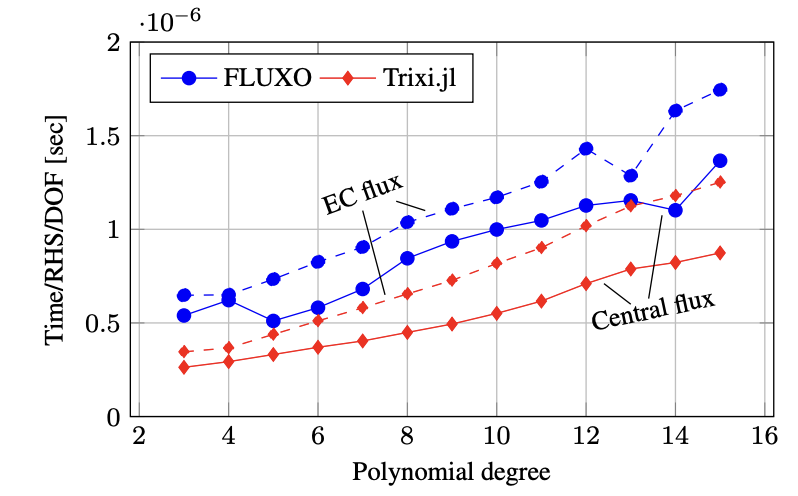
\includegraphics[width=1\linewidth]{abs.png}
        \caption{Absolute run times}
        \label{fig:figure1}
    \end{subfigure}%
    \begin{subfigure}{0.5\textwidth} % Place the second subfigure in the other half of the text width
        \centering
        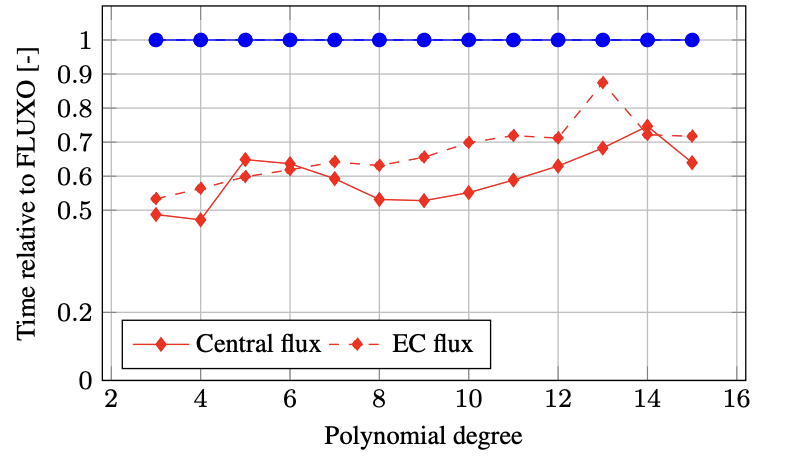
\includegraphics[width=1\linewidth]{rel.png}
        \caption{Run time relative to FLUXO}
        \label{fig:figure2}
        \cite{ranocha2021adaptive}
    \end{subfigure}
    \caption{: Run time per right-hand side evaluation and degree of freedom for
the flux differencing DG discretization of the 3D ideal MHD equations.
Two configurations are compared using either the central volume flux (algebraically equivalent to the weak form DG solver) and the entropy conservative (EC) volume flux.}
    \label{fig:combined}
\end{figure}
\begin{table}[H]
\centering
\caption{Maximum and minimum velocities along the center lines with different weight ratios of residual loss and the boundary loss.}
\begin{tabular}{ccccccccc}
\toprule
$\frac{\omega_R}{\omega_{BC}}$ & $Ra = 10^3$ & & & $Ra = 10^4$ & & & $Ra = 10^5$ \\
\cmidrule{2-3} \cmidrule{5-6} \cmidrule{8-9}
& $u_{\text{max}}$ & $v_{\text{max}}$ & & $u_{\text{max}}$ & $v_{\text{max}}$ & & $u_{\text{max}}$ & $v_{\text{max}}$ \\
\midrule
0.5 & 0.137 & 0.138 & 0.190 & 0.231 & 0.137 & 0.273 \\
1 & 0.192 & 0.233 & 0.128 & 0.258 & & \\
2 & 0.132 & 0.261 & & & & \\
4 & 0.130 & 0.261 & & & & \\
\bottomrule
\end{tabular}
\end{table}
\printbibliography
\end{document}
